\documentclass[tikz,border=10pt]{standalone}
\begin{document}
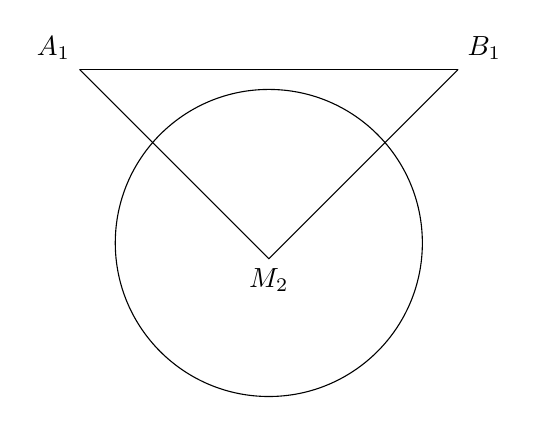
\begin{tikzpicture}[line join=round, line cap=round]

\coordinate (A1) at (-2.4,2.4);
\coordinate (B1) at (2.4,2.4);
\coordinate (M2) at (0,0);

\draw (A1) -- (B1);
\draw (A1) -- (M2);
\draw (B1) -- (M2);
\draw (0,0.2) circle[radius=1.95];

\node[above left] at (A1) {$A_1$};
\node[above right] at (B1) {$B_1$};
\node[below] at (M2) {$M_2$};

\end{tikzpicture}
\end{document}
